\documentclass{beamer}

\usepackage[utf8]{inputenc}
\usepackage[T1]{fontenc}
\usepackage{textcomp,hyperref,multicol}
\usepackage{times}

\usetheme{Frankfurt}
\usecolortheme{orchid}

\usepackage{color}
\title{How social media affect FOSS}
\subtitle{INF5780 Project 2}
\author{{John Rongved} \and {Lars Tveito} \and {Kristian A. Hiorth}}
\date{November 13, 2014}

\institute{Department of Informatics\\University of Oslo}

% fits the presentation to the window when first displayed
\hypersetup{pdfstartview={Fit}}

%% \AtBeginSection[]{%
%%   \begin{frame}<beamer>{Outline}
%%     \tableofcontents[currentsection,currentsubsection]
%%   \end{frame}
%% }

\newcommand{\coloreddot}[1][black]{\Large\textcolor{#1}{\ensuremath\bullet}}
\setbeamertemplate{caption}{\raggedright\insertcaption\par}

\begin{document}


\begin{frame}
  \titlepage
\end{frame}

\begin{frame}{Outline}
  \tableofcontents{}
\end{frame}

\section{Motivation}

%\subsection{Inspiration}

\begin{frame}{Inspiration}
  %\begin{center}
  \begin{figure}
    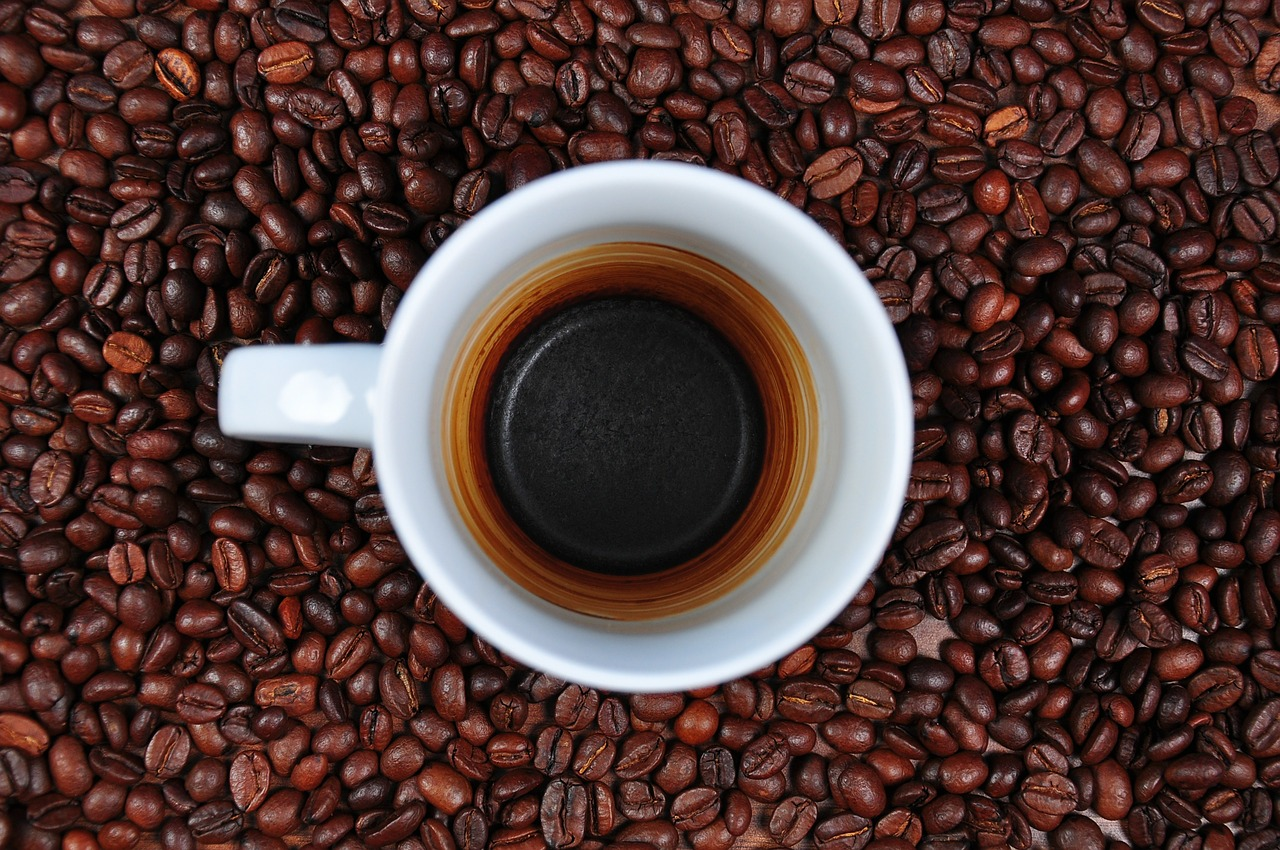
\includegraphics[width=.6\textwidth]{coffee.jpg}
    %\caption{We had coffee}
  \end{figure}
  %% \begin{itemize}
  %%   \item
  %% \end{itemize}
\end{frame}

\begin{frame}
  \begin{multicols}{2}

    \begin{center}
      
\includegraphics[width=.35\textwidth]{Reddit_logo.pdf}

      \vskip5em

      
\includegraphics[width=.35\textwidth]{hacker-news_logo.jpg}
    \end{center}

    \begin{center}
      
\includegraphics[width=.35\textwidth]{so-logo.eps}

      \vskip5em

      
\includegraphics[width=.35\textwidth]{GitHub_Logo.eps}
    \end{center}
  \end{multicols}
  \vskip2em
  \begin{center}
    All of us used these sites
  \end{center}
\end{frame}

%\subsection{Research Topic}

\begin{frame}{Research Topic}
  \begin{itemize}
    %% \item Free and Open Source Software (FOSS) projects are a kind of Community
    %%   Based Peer Production (CBPP)
    %% \item They revolve around a community
    %% \item Social Media has changed how Internet
    %%   communities work
  \item FOSS/CBPP is community based
  \item Social media affect internet communities
  \item How does social media affect FOSS?
    %% \item We wanted to investigate how Social Media have been, and are,
    %%   influencing FOSS projects in particular
  \end{itemize}
\end{frame}

%\subsection{Key Aspects of FOSS Projects}

\begin{frame}{Key Aspects}
  Exposure
  \begin{itemize}
  \item Needed to attract both users and contributors
  \end{itemize}
  \pause
  Knowledge base
  \begin{itemize}
  \item A mechanism for distributing knowledge resources.
    %% \item Like all software, FOSS has to be supported.
  \end{itemize}
  \pause
  Development tools
  \begin{itemize}
  \item Complex structures demands simplifying tools
    %% \item Developers need good tools
  \item Collaboration tools are essential for scalable projects
    %% \item Internal communication and coordination of tasks is
    %% \item FOSS developers are usually distributed spatially,
    %%   compounding the need for efficient tools
  \end{itemize}
\end{frame}

%\subsection{Relevant Social Media Sites}

\begin{frame}{Social News}
  \begin{center}
    
\includegraphics[width=.6\textwidth]{Reddit_logo.pdf}

    \vskip0pt plus.5fill

    
\includegraphics[width=.6\textwidth]{hacker-news_logo.jpg}
  \end{center}
\end{frame}


\begin{frame}{Social Q \& A}
  \begin{center}
    
\includegraphics[width=.6\textwidth]{so-logo.eps}
  \end{center}
\end{frame}

\begin{frame}{Social Coding}
  \begin{center}
    
\includegraphics[width=.6\textwidth]{GitHub_Logo.eps}
  \end{center}
\end{frame}

\section{Related work}

%\subsection{Social coding}

\begin{frame}{GitHub vs Sourceforge}
  \begin{figure}
    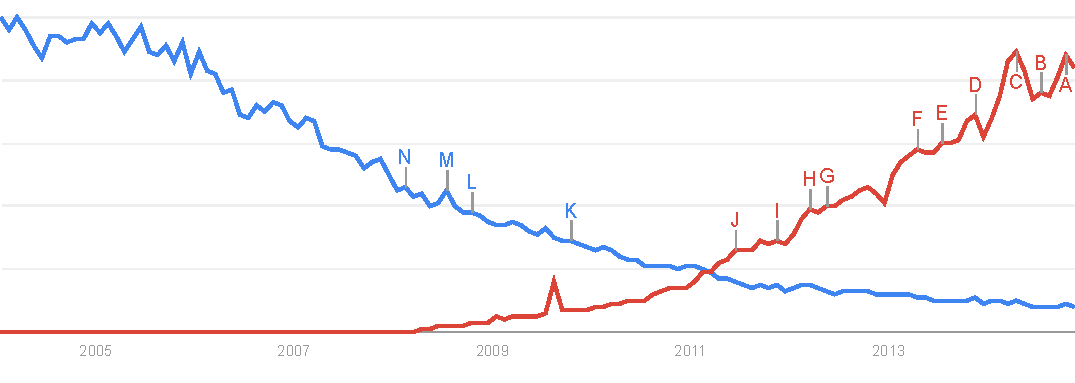
\includegraphics[width=\textwidth]{sourceforge-github.pdf} \\
    \caption{\coloreddot[red] Github \hspace{2em} \coloreddot[blue] Sourceforge\footnote{\href{http://www.google.com/trends/explore\#q=sourceforge\%2C\%20github\&cmpt=q}{Source: Google Trends}}}
  \end{figure}
\end{frame}


%\subsection{Social Q \&{} A}

%\subsection{Social news}

\section{Discussion}

\begin{frame}
  Trends indicate there is a relationship between these sites
  \begin{itemize}
  \item Supported by litterature\footnote{Vasilescu et al. 2014}
  \item Supported by Internet analytic tools\footnote{alexa.com and similarweb.com}
  \end{itemize}
  Similarities between the sites
  \begin{itemize}
  \item Extensive use of gamification
  \item Encouraging participation, creation and promotion of high-quality content
  \end{itemize}
\end{frame}

\begin{frame}[allowframebreaks]{Outreach}
  Social Media traffic patterns
  \begin{itemize}
  \item Wanted to look for evidence of reddit/HN influence on GitHub
  \item Reached out to GitHub about access to traffic data
  \item Could not share any for privacy reasons
    \end{itemize}

  \framebreak
  
  Attempted the social approach ourselves:
  \begin{itemize}
  \item Posted\footnotemark{} to \texttt{/r/emacs}
    about migrating Emacs project to GitHub
  \item Interesting discussion ensued
  \end{itemize}
  \footnotetext{\href{http://goo.gl/MwwiQ0}{http://goo.gl/MwwiQ0}}

\end{frame}

\begin{frame}{Benefits}
  Biggest benefits likely for small and emerging projects
  \begin{itemize}
  \item Lack established ``brand names'' when seeking exposure
  \item Attractive to those wanting attention as contributors
    \item Crosspollination between projects a success
      factor\footnote{Singh et al. 2011}
  \end{itemize}
  
  But also for mature projects
  \begin{itemize}
  \item Lower treshold for engaging with community
  \item New modules can be started independently
  \end{itemize}
\end{frame}

\begin{frame}{Hazards}
  It's not \emph{all} unicorns and rainbows

  \begin{itemize}
  \item Lack of control, danger of lock-in
  \item Unclear ownership of, rights to data
  \item Gamification and crowd moderation fallout
  \end{itemize}
\end{frame}

\section*{Summary}

\begin{frame}{Summary}
  Social Media...
  \begin{itemize}
  \item Can have CBPP-like elements (user driven content)
  \item Provide new community dynamics interesting to FOSS
    projects
  \item Should be approached with heed
  \end{itemize}


  \pause
  \vskip0pt plus.5fill

  Questions?
\end{frame}

\appendix
\section<presentation>*{\appendixname}
\subsection<presentation>*{References}

\begin{frame}
  \frametitle<presentation>{References}
    
  \begin{thebibliography}{10}
    
  \beamertemplatearticlebibitems
  % Followed by interesting articles. Keep the list short.

\bibitem{Vasilescu2014}
  B .Vasilescu, A. Serebrenik, P. Devanbu, and V. Filkov.
  \newblock ``How Social Q\&A Sites Are Changing Knowledge Sharing in
  Open Source Software Communities''
 \newblock {\em Proceedings of the 17th ACM Conference on Computer
   Supported Cooperative Work \& Social Computing}, (2014), pp. 342-354.

  \bibitem{Singh2011}
    P. V. Singh, Y. Tan, and V. S. Mookerjee.

 \newblock ``Network Effects: The Influence of Structural Capital on Open Source Project Success''.
    \newblock {\em MIS Quarterly}, 35.4 (2011), pp. 813-829.
  \end{thebibliography}

  \vskip0pt plus.5fill
  Full bibliography in the essay.
\end{frame}

\end{document}
